% !TeX root = ../main.tex

\chapter{实验设计、结果与分析}
\label{cha:experiment}

\section{实验目标与证据边界}
\label{sec:exp-goal}

本章实验围绕三个层级的问题展开。第一，基于基准忠实协议验证选择性混合路由是否能够在受限云调用下提升长尾场景感知效果；第二，基于适配评估协议分析结构化技能沉淀与复用是否具有独立机制价值；第三，通过真实数据试验讨论本文方法的外部效度与局限性。三类实验分别服务于强结论、机制结论和观察结论，彼此之间不互相替代。

这一安排的目的在于保持论断与证据强度一致。主实验回答的是“系统在线路径是否有效”；独立适配实验回答的是“外部知识复用是否具有潜力及风险”；真实数据试验回答的是“当前原型在真实分布中暴露出哪些边界”。因此，本文在实验叙事上不将三类结果混合为单一胜利结论，而是分别讨论其所能支撑的问题。

\section{实验设置}
\label{sec:exp-setup}

\subsection{数据集与任务}

主定量实验使用 DTPQA 的 DTP-Synth / Category 1 清洗共享子集。该任务聚焦行人存在性判断，能够直接揭示边缘模型在远距离目标上的假阴性问题\cite{theodoridis2025dtpqa,theodoridis2025evaluating}。在当前主实验中，共享样本数为 50，其中远距离样本 15 个、中距离样本 7 个、近距离样本 21 个、距离未知样本 7 个。该样本划分能够为本文分析“远距离失效是否可被定向补救”提供直接支撑。

此外，本文进一步在 DTP-Real / Category 1 上进行真实数据试验，并使用独立适配数据组织结构化技能复用实验。真实数据试验当前包含 9 个已判定样本，其中远距离样本 3 个、中距离样本 2 个、近距离样本 2 个、距离未知样本 2 个。由于真实试验规模仍较小，因此本文将其定位为外部效度观察，而非主结论来源。

\subsection{对比配置}

本文比较三种系统配置。

\begin{enumerate}
  \item \textbf{边缘单独推理}：仅使用边缘模型完成一次感知。
  \item \textbf{云端单独推理}：使用云端模型直接处理同一输入。
  \item \textbf{选择性混合路由}：以边缘模型为主链路，仅在不确定性或风险规则触发时调用云端纠错。
\end{enumerate}

这三种配置分别代表三种不同研究立场。边缘单独推理代表受限资源下的基础车端能力，云端单独推理代表更强模型上限但忽略系统代价的理想路径，选择性混合路由则代表本文关注的部署导向系统方案。在主实验中，选择性混合路由的云端触发率为 18\%，对应 50 个样本中的 9 次云端纠错调用。由于主实验采用基准忠实协议，结构化技能不参与持久化复用。

\subsection{模型与实现条件}

边缘模型采用参数规模相对可控的开源视觉语言模型，云端模型采用更强的多模态模型服务，嵌入模型用于技能检索表示。需要强调的是，本文中的“边缘”与“云端”首先指代角色分层与推理路径分层，而非真实车端硬件与远程服务器之间的完全物理切分。因此，本文的时延结果应被理解为原型系统中的相对比较结果，真实部署下仍需进一步复测。

在当前论文版本中，硬件环境、模型版本号、推理并发设置、网络条件和批处理策略尚未完整展开，这些信息将直接影响绝对时延解释，因此需在后续定稿阶段补充[需补充实现细节]。不过，本文在同一实验环境下对三种配置进行横向比较，因此相对时延差异仍具有分析价值。

\subsection{评价指标}

为同时反映效果、代价与机制特征，本文采用如下指标。

\begin{enumerate}
  \item \textbf{任务效果指标}：精确匹配准确率、正类召回率、负类特异性和远距离子集准确率。
  \item \textbf{系统代价指标}：平均时延、中位数时延、95 分位时延以及云调用比例。
  \item \textbf{机制分析指标}：错误修复率、正确样本伤害率以及云调用削减比例。
\end{enumerate}

对于统计显著性与置信区间，当前稿件尚未给出完整报告，相关内容将在后续工作中补充[需补充统计显著性检验]。

\subsection{对比方法选择依据}
\label{sec:exp-baseline-rationale}

本文没有引入大量外部复杂基线，而是围绕研究问题选择最具解释性的三类在线路径。其原因在于，本文要回答的并非“不同小模型谁更强”，而是“在固定边缘模型基础上，系统级选择性协同是否有效”。如果将大量不同参数规模、不同训练数据来源、不同多模态接口的模型同时纳入主表，反而会削弱本文关于系统组织方式的核心论点。因此，主实验更强调同一任务、同一共享样本、不同推理路径之间的公平比较。

\section{与已发表基线的关系}
\label{sec:exp-baseline-align}

本文公开基线主要参考 Theodoridis 等人对 DTPQA 上小型视觉语言模型的系统评测结果\cite{theodoridis2025evaluating}。该工作展示了多个公开模型在完整基准上的表现，可用来说明距离敏感任务对小型模型的挑战。需要指出的是，本文结果来自清洗后的共享子集，而不是与公开工作完全同条件的全量评测。因此，表~\ref{tab:published-baseline} 仅用于说明本文系统在目标子任务上的方向性收益，而不应被解释为完整基准排行榜对比。

\begin{table}[htbp]
  \centering
  \small
  \bicaption{已发表基线与本文系统在目标子任务上的定向比较}{Directional comparison between published baselines and our system on the target subtask}
  \label{tab:published-baseline}
  \begin{tabularx}{\textwidth}{l l c c}
    \toprule
    方法 & 评测范围 & 准确率（\%） & 备注 \\
    \midrule
    Human Performance & DTPQA 原论文结果 & 95.7 & 已发表上限 \\
    Ovis2-2B & DTPQA 全量基准 & 71.5 & 已发表小模型结果 \\
    InternVL2.5-2B-MPO & DTPQA 全量基准 & 71.0 & 已发表结果 \\
    Qwen2-VL-2B & DTPQA 全量基准 & 61.4 & 已发表结果 \\
    Qwen2.5-VL-3B & DTPQA 全量基准 & 17.3 & 已发表结果 \\
    \textbf{本文：边缘单独推理} & 清洗共享子集 & 90.0 & 本文统计 \\
    \textbf{本文：云端单独推理} & 清洗共享子集 & 96.0 & 本文统计 \\
    \textbf{本文：选择性混合路由} & 清洗共享子集 & 98.0 & 本文统计 \\
    \bottomrule
  \end{tabularx}
\end{table}

从表~\ref{tab:published-baseline} 可以看出，本文方法在目标子任务上的结果显著高于已发表小模型基线。这说明，针对距离敏感失效，系统级协同设计可能比简单更换小模型更有效。但由于评测范围并不完全一致，本文不将该结果表述为完整基准最优，也不将其解读为对所有数据分布都成立的普适结论。

\section{主实验：三路系统比较}
\label{sec:exp-main}

\subsection{整体结果}

三种配置在主实验中的核心结果如表~\ref{tab:three-way-main} 所示。

\begin{table}[htbp]
  \centering
  \scriptsize
  \setlength{\tabcolsep}{3.5pt}
  \bicaption{清洗共享子集上的三路主实验结果}{Main three-way comparison on the cleaned shared subset}
  \label{tab:three-way-main}
  \begin{tabularx}{\textwidth}{l c c c c c c c}
    \toprule
    配置 & EM & \shortstack{正类\\召回} & \shortstack{负类\\特异性} & \shortstack{远距离\\准确率} & \shortstack{平均时延\\（ms）} & \shortstack{P50\\（ms）} & \shortstack{P95\\（ms）} \\
    \midrule
    边缘单独推理 & 0.90 & 0.884 & 1.000 & 0.733 & 13765.54 & 13543.53 & 24460.26 \\
    云端单独推理 & 0.96 & 0.953 & 1.000 & 0.867 & 101053.60 & 93006.96 & 174343.51 \\
    选择性混合路由 & \textbf{0.98} & \textbf{0.977} & 1.000 & \textbf{0.933} & 25330.26 & 6704.66 & 127474.50 \\
    \bottomrule
  \end{tabularx}
\end{table}

表~\ref{tab:three-way-main} 表明，边缘单独推理已经具备较强基础能力，但在远距离子集上的退化仍然明显；云端单独推理提供了更高性能上限，但其平均时延超过 \SI{100000}{ms}，难以作为默认主链路；选择性混合路由则在有限云调用下同时取得了最高总体准确率和最高远距离准确率，说明边缘云协同在本文所研究的场景中具备明确的系统价值。

如果从任务表现和系统代价的联合视角看，三种路径分别对应三种典型状态：边缘路径代表低代价但存在长尾脆弱性的基础能力，云端路径代表高能力上限但部署成本过高的理想能力，而选择性混合路由则代表通过有限补救获得综合收益的折中方案。本文的主结果恰恰说明，在共享样本规模并不大的情况下，系统增益主要来自对少量关键样本的正确识别，而非对全部样本进行昂贵重算。

\begin{figure}[htbp]
  \centering
  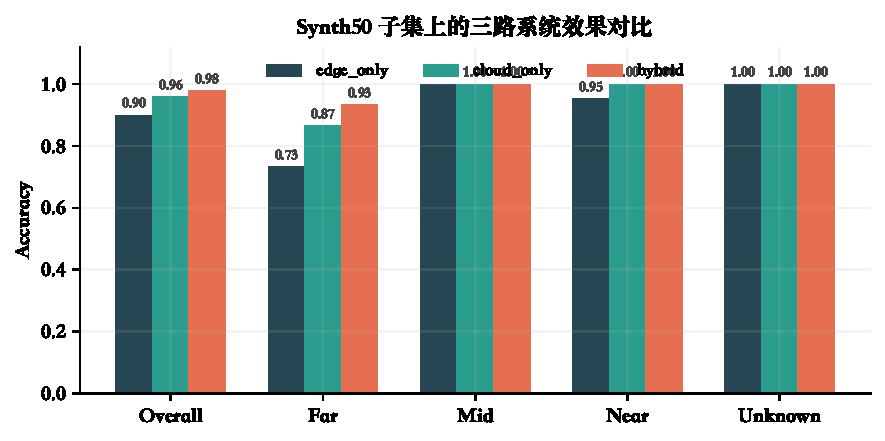
\includegraphics[width=0.95\textwidth]{image/thesis/fig_main_results.pdf}
  \bicaption{整体与分距离准确率比较}{Overall and distance-group accuracy comparison}
  \label{fig:main-results}
\end{figure}

图~\ref{fig:main-results} 进一步显示，三种配置在近距离与中距离样本上的差异有限，而在远距离子集上的差距最为显著。这说明本文方法的主要收益来自对关键脆弱样本的定向补救，而非对所有样本的普遍重写。尤其是在 15 个远距离样本上，边缘路径的准确率仅为 73.3\%，而混合路径提高到 93.3\%，表明系统增益高度集中在本文最关心的高风险失效区域。

\subsection{分距离结果分析}
\label{sec:exp-distance}

从不同距离组的表现可以进一步观察到本文方法的作用机制。对于近距离、中距离和距离未知样本，边缘模型本身已经具有较高稳定性，因此混合路由带来的改善空间有限；而对于远距离样本，边缘模型更容易因为目标尺度过小、有效像素不足或局部证据模糊而给出保守否定判断，此时云端补救能够显著提高正类召回率。换言之，本文方法的收益不是均匀分布在整个输入空间，而是集中作用于原始系统最容易失效的区域。

这一现象与本文的问题设定一致。自动驾驶中的长尾风险往往不是全局平均难度升高，而是局部高风险条件下的集中退化。因此，若系统能够较好地识别这类条件并触发低频高价值纠错，那么即使云端调用比例不高，也可能获得显著的整体收益。

\subsection{系统代价分析}

准确率提升只有在系统代价可接受时才具有部署意义。图~\ref{fig:latency} 给出了三种配置的时延分布统计。

\begin{figure}[htbp]
  \centering
  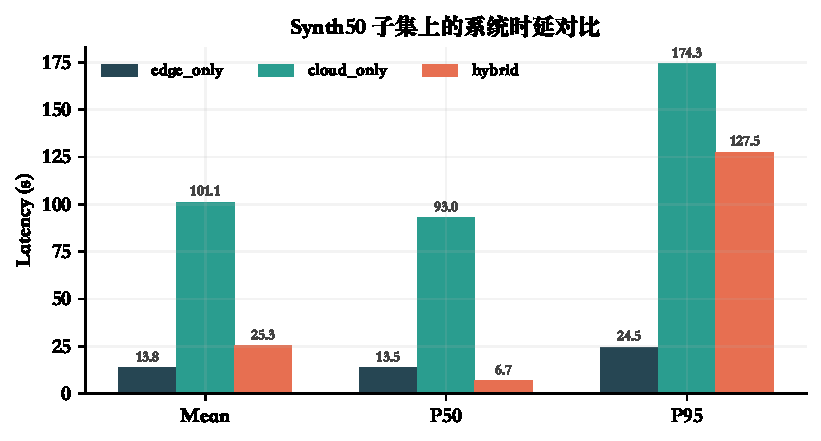
\includegraphics[width=0.90\textwidth]{image/thesis/fig_latency.pdf}
  \bicaption{三种配置的时延统计}{Latency statistics of the three execution modes}
  \label{fig:latency}
\end{figure}

结果表明，云端单独推理在平均时延和长尾时延上均显著高于边缘单独推理；选择性混合路由虽然引入了少量高时延样本，但平均时延仍远低于云端单独推理。在当前实验中，选择性混合路由相较于云端单独推理将云调用比例降低 82\%，平均时延降低 74.9\%，表明其准确率提升并不是由大规模转向云端换得的。

值得注意的是，混合路由的 P95 时延仍然较高，这说明在被触发的个别样本上，云端调用和多阶段流程仍会带来明显的长尾延迟。对此，本文的结论并非“混合路由已经完全满足真实车端实时性要求”，而是“在当前原型条件下，相较于全云路径，选择性协同显著降低了平均系统代价”。真实部署中如何进一步平滑长尾时延，仍需通过更严格的系统工程优化来解决。

\subsection{系统级收益与伤害分析}

为了衡量混合路由是否真正修复了边缘模型的关键错误，本文进一步统计其错误修复率与伤害率，如图~\ref{fig:system-effectiveness} 所示。

\begin{figure}[htbp]
  \centering
  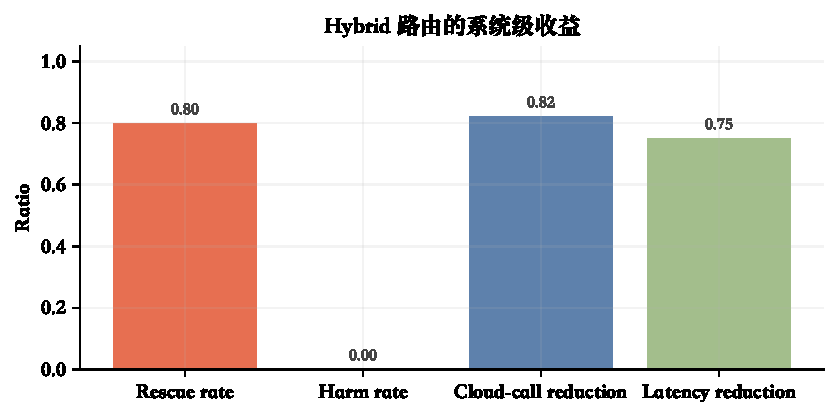
\includegraphics[width=0.85\textwidth]{image/thesis/fig_system_effectiveness.pdf}
  \bicaption{混合路由的系统级收益}{System-level gains of the selective hybrid route}
  \label{fig:system-effectiveness}
\end{figure}

在 50 个样本中，边缘单独推理共出现 5 个错误，选择性混合路由修复了其中 4 个，对应 80\% 的错误修复率；与此同时，选择性混合路由未破坏任何原本正确的样本，伤害率为 0。该结果说明，本文方法并非通过激进修正牺牲保守性来换取收益，而是在相对谨慎的路由条件下提升了关键长尾样本的识别能力。

进一步结合台账统计可以发现，这 4 个被修复的错误中有 3 个来自远距离样本。由此可见，本文方法的有效性并非来自随机纠正，而是与远距离脆弱性这一核心失效模式高度一致。这也从侧面支持了本文关于“系统增益集中于长尾高风险区域”的研究判断。

\section{机制分析与消融讨论}
\label{sec:exp-ablation}

除了主结果外，本文还对混合路由中两个关键机制进行了分析。首先，在早期原型中，若不严格隔离历史知识状态并统一样本集合，混合路由结果会受到跨轮次状态残留的影响，从而高估或低估系统表现。这一现象说明，对于包含外部知识记忆的系统研究，协议洁净性本身就是实验有效性的一部分[需补充更严格的协议对照结果]。

其次，初步诊断表明，仅基于边缘输出进行语言层面的纠错，容易将云端模型锚定在边缘模型的错误解释上；而将纠错过程改为以原始图像为主的图像级再感知后，远距离假阴性样本的修复效果更稳定。该观察与本文方法设计的理论动机一致，即真正需要修复的往往是观察过程，而不仅是语言表达过程。由于当前尚缺少严格配对的同日消融结果，本文在此仅给出机制性解释，并将完整对照实验留作后续补充[需补充图像级纠错与文本级纠错的配对消融]。

此外，当前版本尚缺少对路由阈值、规则触发强度和云调用预算之间关系的系统性敏感性分析。根据现有结果可以初步推断，更激进的触发策略有望进一步提高远距离召回，但也可能显著放大长尾时延和云调用比例；更保守的触发策略则可能损失长尾修复能力。关于这一折中关系，仍需通过完整参数扫描给出定量曲线[需补充参数敏感性分析]。

\section{独立适配实验：结构化技能的收益与风险}
\label{sec:exp-skill}

为了避免将结构化技能复用与主基准结果混写，本文在独立适配协议下单独评估结构化技能的作用，其结果如图~\ref{fig:skill-adaptation} 所示。

\begin{figure}[htbp]
  \centering
  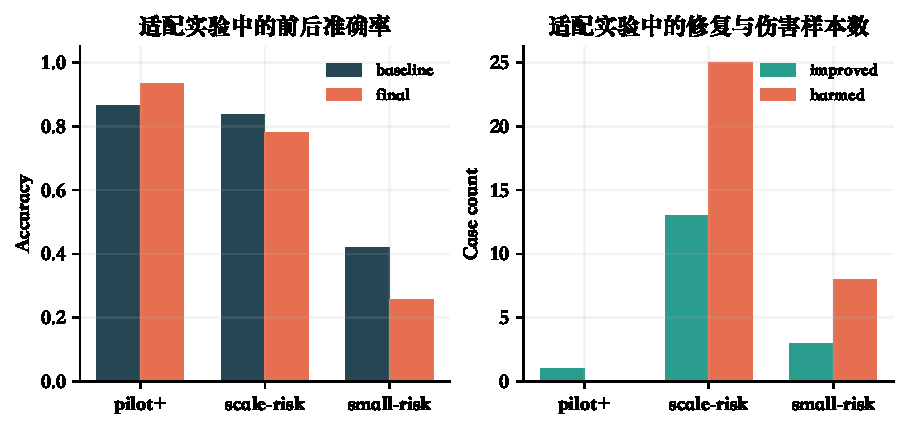
\includegraphics[width=0.95\textwidth]{image/thesis/fig_skill_adaptation.pdf}
  \bicaption{独立适配实验中的收益与风险}{Gains and risks in the independent adaptation experiments}
  \label{fig:skill-adaptation}
\end{figure}

为便于比较，表~\ref{tab:skill-adaptation} 总结了三组独立适配实验的关键统计结果。

\begin{table}[htbp]
  \centering
  \small
  \bicaption{独立适配实验统计汇总}{Summary of the independent adaptation experiments}
  \label{tab:skill-adaptation}
  \begin{tabularx}{\textwidth}{l c c c c c}
    \toprule
    实验配置 & 样本数 & 基线准确率 & 最终准确率 & 修复样本数 & 伤害样本数 \\
    \midrule
    小规模正向闭环 & 15 & 0.8667 & 0.9333 & 1 & 0 \\
    规模扩大风险试验 & 209 & 0.8373 & 0.7799 & 13 & 25 \\
    小样本回退试验 & 31 & 0.4194 & 0.2581 & 3 & 8 \\
    \bottomrule
  \end{tabularx}
\end{table}

结果显示，结构化技能在小规模闭环中可以产生正向收益。例如，在小规模试验中，系统准确率由 0.8667 提升至 0.9333，修复了远距离样本且未引入新的错误。这说明，将纠错经验抽象为结构化知识并用于后续再感知，在机制上是可行的。

然而，当结构化技能复用范围扩大后，系统性能出现回落，并伴随明显的伤害样本增加。这表明，外部知识复用虽然能够带来额外收益，但其稳定性高度依赖检索精度、知识粒度和场景分布匹配程度。从表~\ref{tab:skill-adaptation} 可以看到，在规模扩大风险试验中，虽然有 13 个样本得到修复，但同时有 25 个样本受到伤害；在小样本回退试验中，伤害样本同样超过修复样本。这说明结构化技能不是天然安全的“经验缓存”，而是一种需要严格边界控制的外部知识机制。

结合改进样本的距离分布可以进一步发现，正向收益主要集中在远距离样本，而回退风险则更容易在距离未知或上下文差异较大的样本上暴露。这一现象提示，技能复用的有效性与场景匹配精度密切相关，后续研究需要进一步建立更严格的技能构建集、验证集和评估集划分方式[需补充技能评估协议说明]。

\section{真实数据试验}
\label{sec:exp-real}

真实数据试验主要用于分析方法的外部效度，而不作为主胜利结果。当前 DTP-Real / Category 1 试验的整体准确率为 0.4444，远距离子集准确率为 0，表明真实场景中的远距离失效远比清洗合成子集更为严重。

\begin{figure}[htbp]
  \centering
  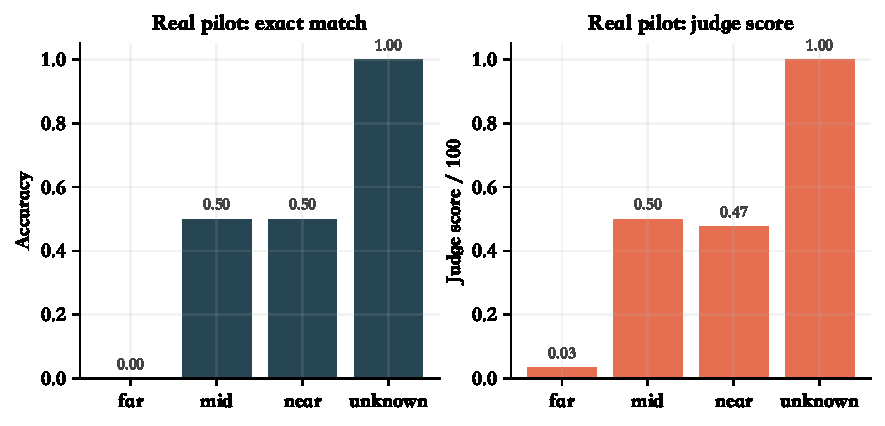
\includegraphics[width=0.88\textwidth]{image/thesis/fig_real_pilot_failure.pdf}
  \bicaption{真实数据试验中的远距离崩塌与假阴性偏置}{Far-collapse and false-negative bias observed in the real-data pilot}
  \label{fig:real-pilot}
\end{figure}

图~\ref{fig:real-pilot} 表明，真实数据中的远距离正样本更容易被误判为否定类别，显示出明显的假阴性偏置。进一步查看距离组统计可知，3 个远距离样本全部判断失败，而距离未知组的 2 个样本则全部回答正确。这说明当前方法并不是“整体不可用”，而是对真实远距离场景存在高度结构化失效。进一步的定向干预试验虽在部分远距离样本上带来了改进，但同时也导致其他子集性能下降，说明当前方法对真实分布仍具有较强敏感性。这一结果提示，清洗后的合成子集并不能替代真实世界评估。

\section{案例分析}
\label{sec:exp-case}

为了更直观地展示系统行为，图~\ref{fig:case-studies} 给出了一组成功案例与失败案例的对照。

\begin{figure}[htbp]
  \centering
  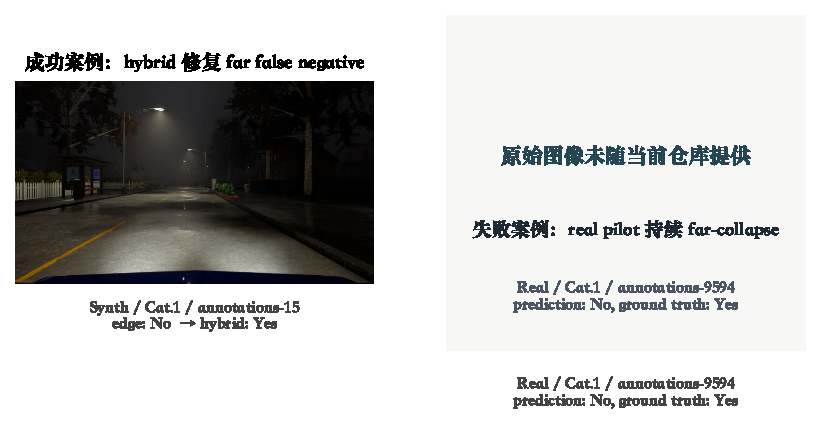
\includegraphics[width=0.95\textwidth]{image/thesis/fig_case_studies.pdf}
  \bicaption{典型成功与失败案例}{Representative success and failure cases}
  \label{fig:case-studies}
\end{figure}

成功案例表明，本文方法能够在边缘模型对远距离目标给出漏判时，通过选择性云协同完成纠正；失败案例则显示，在真实数据中，系统仍可能持续保持过于保守的否定判断。两类案例共同说明，本文方法已经具备针对部分长尾失效的补救能力，但距离稳定覆盖真实世界复杂场景仍有明显差距。

\section{误差分析与稳健性讨论}
\label{sec:exp-error}

综合主实验、独立适配实验与真实数据试验，本文当前方法的误差来源主要体现在三个方面。第一，远距离目标本身的视觉证据不足仍然是最主要的错误根源，尤其在真实场景中表现得更为明显。第二，结构化技能在跨场景复用时容易受到语义近似但上下文不一致样本的干扰，导致知识调用出现“看似匹配、实则误导”的问题。第三，系统当前对路由阈值和云调用预算的调节仍较为粗粒度，当输入分布发生明显变化时，原有触发策略可能不再稳健。

这些误差分析进一步说明，本文方法的价值更多体现在“揭示一种可行的系统组织方式”，而非宣称已经完全解决自动驾驶长尾问题。对于真实部署而言，如何联合考虑视觉证据质量估计、路由稳健性控制和技能污染抑制，将是决定该方法能否进一步走向实用化的关键。

\section{本章小结}
\label{sec:exp-summary}

本章按照主实验、机制分析、独立适配实验、真实数据试验与误差分析的顺序，建立了与证据强度相一致的实验叙事。总体而言，主实验说明选择性混合路由在目标任务上是有效的；独立适配实验说明结构化技能具有机制潜力但尚需进一步约束；真实数据试验与误差分析则揭示了方法在外部世界中的适用边界。
